\documentclass[tikz,border=10pt]{standalone}
\usepackage[T1]{fontenc}
\usepackage{lmodern}
\usepackage{xcolor}
\usepackage{textcomp}
\usepackage{tikz}
\usetikzlibrary{arrows.meta,backgrounds,calc,positioning}

% Muted academic palette
\definecolor{titleblue}{HTML}{294E80}
\definecolor{lineblue}{HTML}{5F86B3}
\definecolor{panelstroke}{HTML}{9FB4CC}
\definecolor{panelfill}{HTML}{F7FAFD}
\definecolor{accent}{HTML}{C96A1B}
\definecolor{accentfill}{HTML}{FBECDD}
\definecolor{rowfill}{HTML}{F3F5F7}
\definecolor{textgray}{HTML}{5E6470}
\definecolor{ink}{HTML}{222222}
\definecolor{dotblue}{HTML}{3A84B7}
\definecolor{dotgreen}{HTML}{4E9A61}
\definecolor{dotpurple}{HTML}{7B5AA6}

\tikzset{
  panel/.style={
    rounded corners=7pt,
    draw=panelstroke,
    line width=1pt,
    fill=panelfill
  },
  phase/.style={
    rectangle,
    rounded corners=4pt,
    fill=titleblue,
    text=white,
    font=\rmfamily\bfseries\small,
    minimum width=4.7cm,
    minimum height=7.5mm
  },
  connector/.style={
    rectangle,
    rounded corners=4pt,
    fill=lineblue,
    text=white,
    font=\rmfamily\bfseries\small,
    minimum width=2.8cm,
    minimum height=6.8mm
  },
  arr/.style={-{Stealth[length=7pt,width=6pt]}, line width=1.35pt, draw=accent},
  arrsoft/.style={-{Stealth[length=6pt,width=5pt]}, line width=1.1pt, draw=lineblue},
  steplabel/.style={font=\rmfamily\bfseries\small, text=ink, align=center},
  stepnote/.style={font=\rmfamily\fontsize{8.4}{10.1}\selectfont, text=textgray, align=center},
  tablehead/.style={font=\rmfamily\bfseries\scriptsize, text=ink},
  tinytext/.style={font=\rmfamily\scriptsize, text=ink},
  cue/.style={font=\rmfamily\bfseries\small, text=titleblue, align=left},
  cuenote/.style={font=\rmfamily\fontsize{7.5}{9}\selectfont, text=textgray, align=left}
}

\begin{document}
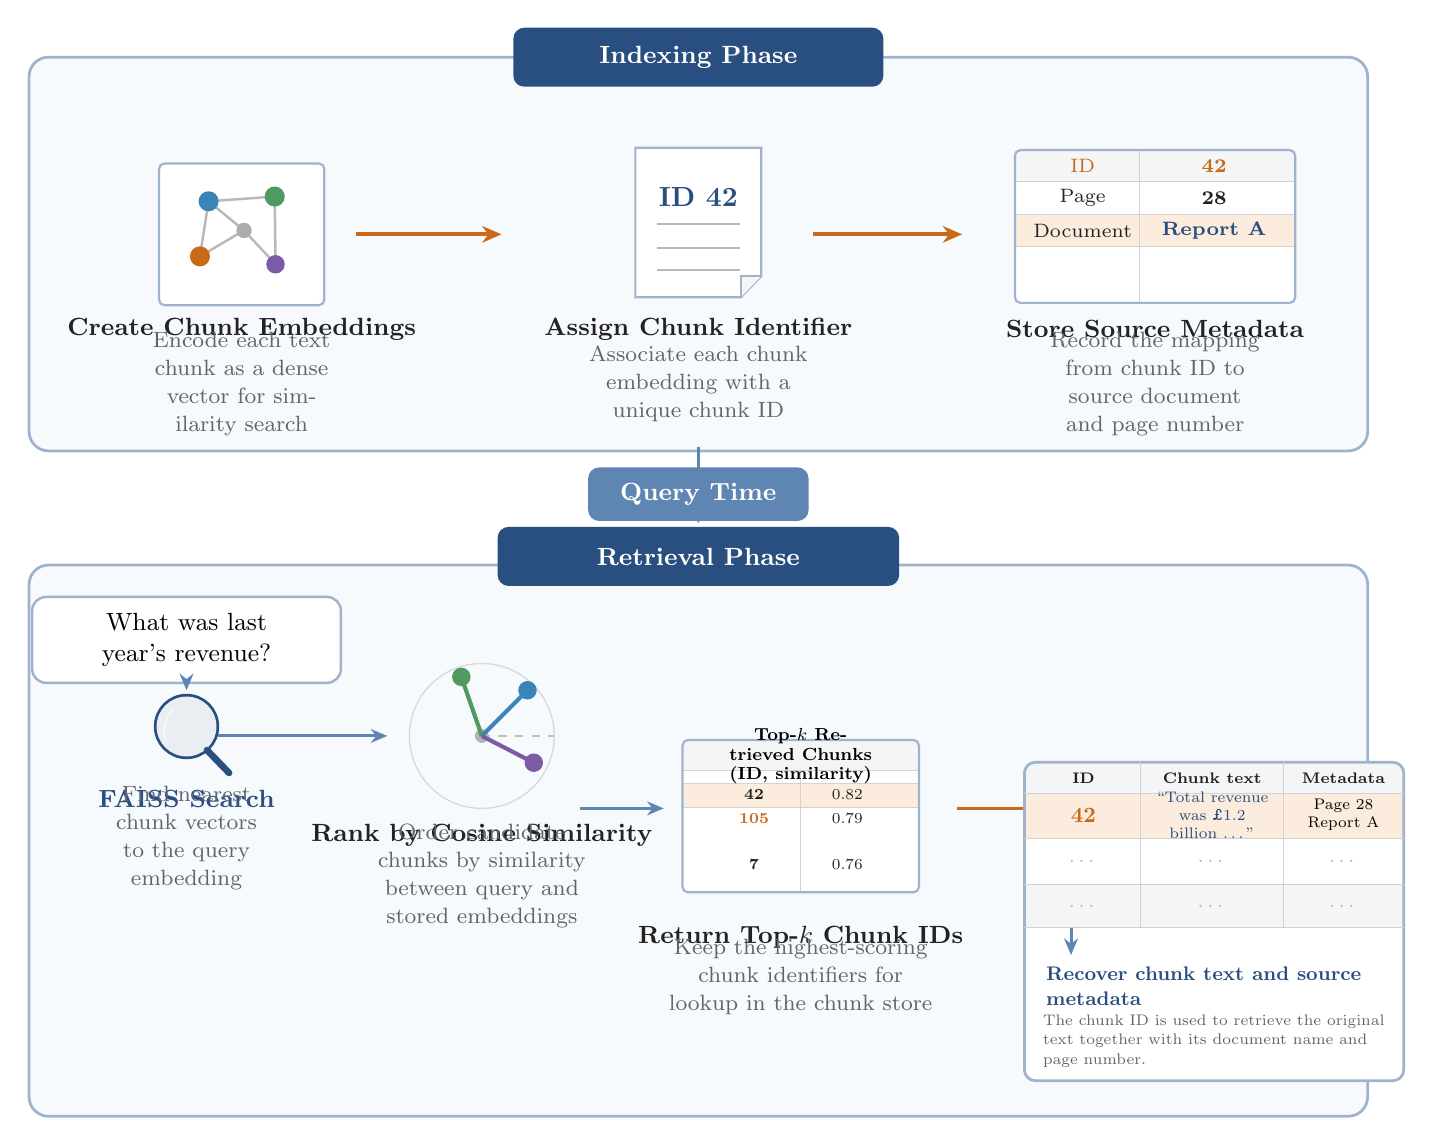
\begin{tikzpicture}[font=\rmfamily]

% Indexing phase
\node[phase] at (9.0, 13.9) {Indexing Phase};
\begin{scope}[on background layer]
  \node[panel, minimum width=17.0cm, minimum height=5.0cm] at (9.0, 11.4) {};
\end{scope}

% Create embeddings
\begin{scope}[shift={(3.2,11.65)}]
  \draw[fill=white, draw=panelstroke, rounded corners=2pt, line width=0.8pt]
    (-1.05,-0.9) rectangle (1.05,0.9);
  \draw[gray!55, line width=0.9pt] (-0.42,0.42)--(0.42,0.48);
  \draw[gray!55, line width=0.9pt] (-0.42,0.42)--(0.03,0.05);
  \draw[gray!55, line width=0.9pt] (0.42,0.48)--(0.43,-0.38);
  \draw[gray!55, line width=0.9pt] (-0.53,-0.28)--(0.03,0.05);
  \draw[gray!55, line width=0.9pt] (0.03,0.05)--(0.43,-0.38);
  \draw[gray!55, line width=0.9pt] (-0.53,-0.28)--(-0.42,0.42);
  \filldraw[dotblue]   (-0.42,0.42) circle(0.12);
  \filldraw[dotgreen]  (0.42,0.48) circle(0.12);
  \filldraw[accent]    (-0.53,-0.28) circle(0.12);
  \filldraw[dotpurple] (0.43,-0.38) circle(0.11);
  \filldraw[gray!65]   (0.03,0.05) circle(0.09);
\end{scope}
\node[steplabel] at (3.2,10.45) {Create Chunk Embeddings};
\node[stepnote, text width=3.0cm] at (3.2,9.75)
  {Encode each text chunk as a dense vector for similarity search};

\draw[arr] (4.65,11.65) -- (6.5,11.65);

% Assign ID
\begin{scope}[shift={(9.0,11.8)}]
  \draw[fill=white, draw=panelstroke, line width=0.8pt]
    (-0.8,-0.95) -- (0.54,-0.95) -- (0.8,-0.68) -- (0.8,0.95) -- (-0.8,0.95) -- cycle;
  \fill[rowfill] (0.54,-0.95) -- (0.54,-0.68) -- (0.8,-0.68) -- cycle;
  \draw[panelstroke, line width=0.55pt] (0.54,-0.95)--(0.54,-0.68)--(0.8,-0.68);
  \node[font=\rmfamily\bfseries\normalsize, text=titleblue] at (0,0.32) {ID 42};
  \draw[gray!55, line width=0.6pt] (-0.52,-0.02)--(0.53,-0.02);
  \draw[gray!55, line width=0.6pt] (-0.52,-0.32)--(0.53,-0.32);
  \draw[gray!55, line width=0.6pt] (-0.52,-0.60)--(0.53,-0.60);
\end{scope}
\node[steplabel] at (9.0,10.45) {Assign Chunk Identifier};
\node[stepnote, text width=3.0cm] at (9.0,9.75)
  {Associate each chunk embedding with a unique chunk ID};

\draw[arr] (10.45,11.65) -- (12.35,11.65);

% Store metadata
\begin{scope}[shift={(14.8,11.6)}]
  \begin{scope}
    \clip[rounded corners=2pt] (-1.78,-0.82) rectangle (1.78,1.12);
    \fill[white] (-1.78,-0.82) rectangle (1.78,1.12);
    \fill[rowfill] (-1.78,0.72) rectangle (1.78,1.12);
    \fill[accentfill] (-1.78,-0.10) rectangle (1.78,0.30);
  \end{scope}
  \draw[gray!35, line width=0.5pt] (-0.2,-0.82)--(-0.2,1.12);
  \draw[gray!35, line width=0.45pt] (-1.78,0.72)--(1.78,0.72);
  \draw[gray!35, line width=0.45pt] (-1.78,0.30)--(1.78,0.30);
  \draw[gray!35, line width=0.45pt] (-1.78,-0.10)--(1.78,-0.10);
  \draw[panelstroke, rounded corners=2pt, line width=0.8pt] (-1.78,-0.82) rectangle (1.78,1.12);
  \node[tinytext, text=accent] at (-0.92,0.92) {ID};
  \node[tablehead, text=accent] at (0.75,0.92) {42};
  \node[tinytext] at (-0.92,0.51) {Page};
  \node[tablehead] at (0.75,0.51) {28};
  \node[tinytext] at (-0.92,0.10) {Document};
  \node[tablehead, text=titleblue] at (0.75,0.10) {Report A};
\end{scope}
\node[steplabel] at (14.8,10.45) {Store Source Metadata};
\node[stepnote, text width=3.2cm] at (14.8,9.75)
  {Record the mapping from chunk ID to source document and page number};

% Query-time connector
\draw[arrsoft] (9.0,8.95) -- (9.0,7.98);
\node[connector] at (9.0,8.35) {Query Time};

% Retrieval phase
\node[phase, minimum width=5.1cm] at (9.0,7.56) {Retrieval Phase};
\begin{scope}[on background layer]
  \node[panel, minimum width=17.0cm, minimum height=7.0cm] at (9.0,3.95) {};
\end{scope}

% Query bubble
\node[
  draw=panelstroke,
  fill=white,
  rounded corners=5pt,
  line width=0.9pt,
  font=\rmfamily\small,
  inner sep=6pt,
  text width=3.5cm,
  align=center
] (query) at (2.5,6.5) {What was last year's revenue?};
\draw[arrsoft] (query.south) -- (2.5,5.86);

% FAISS icon
\begin{scope}[shift={(2.5,5.28)}]
  \draw[titleblue, line width=2pt] (0,0.12) circle(0.38);
  \fill[titleblue!10] (0,0.12) circle(0.38);
  \draw[white, line width=0.8pt, opacity=0.55]
    (-0.15,0.35) arc[start angle=130,end angle=200,radius=0.38];
  \draw[titleblue, line width=2.4pt, line cap=round] (0.26,-0.18)--(0.54,-0.47);
\end{scope}
\node[steplabel, text=titleblue] at (2.5,4.48) {FAISS Search};
\node[stepnote, text width=2.2cm] at (2.5,3.98)
  {Find nearest chunk vectors to the query embedding};

\draw[arrsoft] (2.9,5.28) -- (5.05,5.28);

% Similarity search
\begin{scope}[shift={(6.25,5.28)}]
  \draw[gray!30, line width=0.5pt] (0,0) circle(0.92);
  \filldraw[gray!60] (0,0) circle(0.08);
  \draw[gray!50, dashed, line width=0.65pt] (0,0)--(0.92,0);
  \draw[dotblue, line width=1.5pt] (0,0)--(0.58,0.58);
  \draw[dotgreen, line width=1.5pt] (0,0)--(-0.26,0.75);
  \draw[dotpurple, line width=1.5pt] (0,0)--(0.66,-0.34);
  \filldraw[dotblue] (0.58,0.58) circle(0.11);
  \filldraw[dotgreen] (-0.26,0.75) circle(0.11);
  \filldraw[dotpurple] (0.66,-0.34) circle(0.11);
\end{scope}
\node[steplabel] at (6.25,4.02) {Rank by Cosine Similarity};
\node[stepnote, text width=3.0cm] at (6.25,3.50)
  {Order candidate chunks by similarity between query and stored embeddings};

\draw[arrsoft] (7.5,4.36) -- (8.56,4.36);

% Top-k table
\begin{scope}[shift={(10.3,4.36)}, scale=0.79, transform shape]
  \begin{scope}
    \clip[rounded corners=2pt] (-1.9,-1.35) rectangle (1.9,1.1);
    \fill[white] (-1.9,-1.35) rectangle (1.9,1.1);
    \fill[rowfill] (-1.9,0.61) rectangle (1.9,1.1);
    \fill[accentfill] (-1.9,0.02) rectangle (1.9,0.40);
  \end{scope}
  \draw[gray!35, line width=0.5pt] (0,-1.35)--(0,0.61);
  \draw[gray!35, line width=0.45pt] (-1.9,0.61)--(1.9,0.61);
  \draw[gray!35, line width=0.45pt] (-1.9,0.40)--(1.9,0.40);
  \draw[gray!35, line width=0.45pt] (-1.9,0.02)--(1.9,0.02);
  \draw[panelstroke, rounded corners=2pt, line width=0.8pt] (-1.9,-1.35) rectangle (1.9,1.1);
  \node[font=\rmfamily\bfseries\fontsize{7.7}{9}\selectfont, align=center, text width=3.2cm] at (0,0.84)
    {Top-$k$ Retrieved Chunks\\(ID, similarity)};
  \node[tablehead] at (-0.75,0.23) {42};
  \node[tinytext] at (0.75,0.23) {0.82};
  \node[tablehead, text=accent] at (-0.75,-0.17) {105};
  \node[tinytext] at (0.75,-0.17) {0.79};
  \node[tablehead] at (-0.75,-0.90) {7};
  \node[tinytext] at (0.75,-0.90) {0.76};
\end{scope}
\node[steplabel] at (10.3,2.72) {Return Top-$k$ Chunk IDs};
\node[stepnote, text width=3.4cm] at (10.3,2.22)
  {Keep the highest-scoring chunk identifiers for lookup in the chunk store};

\draw[arr] (12.28,4.36) -- (13.45,4.36);

% Lookup table
\begin{scope}[shift={(15.55,3.84)}, scale=0.79, transform shape]
  \begin{scope}
    \clip[rounded corners=4pt] (-3.05,-3.72) rectangle (3.05,1.4);
    \fill[white] (-3.05,-3.72) rectangle (3.05,1.4);
    \fill[rowfill] (-3.05,0.90) rectangle (3.05,1.4);
    \fill[accentfill] (-3.05,0.18) rectangle (3.05,0.90);
    \fill[rowfill] (-3.05,-1.26) rectangle (3.05,-0.56);
  \end{scope}
  \draw[panelstroke, rounded corners=4pt, line width=1pt] (-3.05,-3.72) rectangle (3.05,1.4);
  \draw[gray!35, line width=0.5pt] (-1.18,-1.26)--(-1.18,1.4);
  \draw[gray!35, line width=0.5pt] (1.12,-1.26)--(1.12,1.4);
  \draw[gray!35, line width=0.45pt] (-3.05,0.90)--(3.05,0.90);
  \draw[gray!35, line width=0.45pt] (-3.05,0.18)--(3.05,0.18);
  \draw[gray!35, line width=0.45pt] (-3.05,-0.56)--(3.05,-0.56);
  \draw[gray!35, line width=0.45pt] (-3.05,-1.26)--(3.05,-1.26);
  \node[tablehead] at (-2.1,1.14) {ID};
  \node[tablehead] at (-0.03,1.14) {Chunk text};
  \node[tablehead] at (2.08,1.14) {Metadata};
  \node[font=\rmfamily\bfseries\normalsize, text=accent] at (-2.1,0.55) {42};
  \node[font=\rmfamily\fontsize{7}{8.3}\selectfont, align=center, text width=2.15cm, text=titleblue] at (-0.03,0.55)
    {``Total revenue was \textsf{\textsterling}1.2 billion \ldots''};
  \node[font=\rmfamily\fontsize{7}{8.3}\selectfont, align=center, text width=1.9cm] at (2.08,0.55)
    {Page 28\\Report A};
  \node[font=\rmfamily, text=gray!55] at (-2.1,-0.20) {\ldots};
  \node[font=\rmfamily, text=gray!55] at (-0.03,-0.20) {\ldots};
  \node[font=\rmfamily, text=gray!55] at (2.08,-0.20) {\ldots};
  \node[font=\rmfamily, text=gray!55] at (-2.1,-0.91) {\ldots};
  \node[font=\rmfamily, text=gray!55] at (-0.03,-0.91) {\ldots};
  \node[font=\rmfamily, text=gray!55] at (2.08,-0.91) {\ldots};
  \draw[arrsoft] (-2.3,-1.26) -- (-2.3,-1.70);
  \node[cue, text width=5.7cm] at (0.15,-2.20) {Recover chunk text and source metadata};
  \node[cuenote, text width=5.8cm] at (0.15,-3.08)
    {The chunk ID is used to retrieve the original text together with its document name and page number.};
\end{scope}

\end{tikzpicture}
\end{document}
